\documentclass[../main.tex]{subfiles}
\begin{document}

\tags{
    \nameref{hc:dataviz},
    \nameref{hc:correlation},
    \nameref{hc:testability},
    \nameref{hc:medium},
    \nameref{hc:professionalism}
}{
    \LOref{CausalBenchmarkDesign},
    \LOref{CodeImplementation}
}

\vspace{\baselineskip}

This chapter presents results and analyses that provide initial validation of the approach, and the implementation, of the Maccabee package. The content is split into two sections corresponding to the two aspects of Maccabee's design that require validation. The first section presents the results aimed at validating the DGP sampling parameterization. This section demonstrates that Maccabee is able to sample DGPs from specified locations in the distributional problem space. The second section presents results aimed at validating Maccabee's benchmarking approach by constructing a series of comparisons between results from Maccabee and results from approaches in the literature. Note that `validation' of basic operational correctness is not covered here. The demonstrations and examples presented throughout the \href{\RTDurl/usage.html}{tutorials} in the package documentation serve to validate this basic aspect of package correctness.

\vspace{\baselineskip}

It is worth noting, explicitly, that validating this package with any level of certainty is a hard problem. First, and most generally, because there is no good way to objectively and quantitatively compare different benchmarking approaches. Producing different results for some method relative to other benchmarking approaches is not indicative of relative superiority/inferiority without a deeper understanding of why the results differ. IE, metric values are directly comparable for different estimators tested on the same benchmark, but they are not directly comparable for the same estimator tested \textit{across} different benchmarks. Differences in metric results, or new information provided by new approaches, are only useful if supported by a credible theoretical understanding of why the results differ or why the new information is important. To this end, the results below rely heavily on the theoretical understanding of causal inference estimators and benchmarking established Chapters \ref{chap:problemspace} and \ref{chap:litreview}.

\vspace{\baselineskip}

Second, as the reader will see below, validating the Maccabee approach relies on quantifying the position of sampled DGPs in the distributional problem space by using the set of \textit{data metrics} that were introduced in Chapter \ref{chap:macdesign}. As discussed when they were first introduced, these metrics are only approximate/imprecise measurements of the true distributional setting of a DGP. In fact, \textcite{Dorie2019Automated1} find almost no correlation between the metrics they propose (the same ones used in this work) and estimator performance even though estimator performance is strongly correlated with the parameterization that they used to control distributional setting in their paper. This means the changes in the distributional setting created by different parameterization of the DGP sampling process are not clearly reflected in changes in the value of metrics. The first section below relies, unavoidably, on the metrics. However, in the second section, I have made an effort to present results that are fairly independent of the data metrics.

\section{Validating the DGP Sampling Parameterization}
\label{sec:validation-dgp-sampling}

Chapter \ref{chap:macdesign} established that one of Maccabee's key design goals is to allow the sampling of DGPs from specified locations in the distributional problem space through the use of a parameterized DGP sampling procedure. Chapter \ref{chap:macimplementation}, and the documentation linked therein, discussed the different ways in which the parameters of the sampling process can be specified by the user. These can be summarized as either \textit{preset} - specifying parameters by selecting a \textit{high}, \textit{medium}, or \textit{low} level on each supported axis of the problem space and then using the low-level parameter values corresponding to each level that are supplied with the package. Or, \textit{customized} - specifying the low-level parameter values directly. This section focuses on validating the parameterization scheme using the first specification approach. If custom low-level parameters are required, users should follow the advanced tutorials in the \RTDlink{package documentation} in order to refine parameter values using the relevant data metrics.

\vspace{\baselineskip}

Figure \ref{fig:sampling-validation-results-1} displays the primary DGP sampling validation results. Each subplot corresponds to a single axis of the problem space. The Y-axis is the value of a metric that measures the location of sampled DGPs along the problem space axis, and the X-axis is the user-specified target \textit{level} for the axis. In each plot, the parameters corresponding to all other axis are kept at package default values. The metric value at each level is evaluated by sampling 32 DGPs and then sampling 100 datasets from each DGP. The value of the data metric is averaged across the datasets for each DGP and then averaged across all DGPs. The error bars correspond to the standard deviation of the metric value between DGPs.

\begin{figure}[ht!]
    \centering
    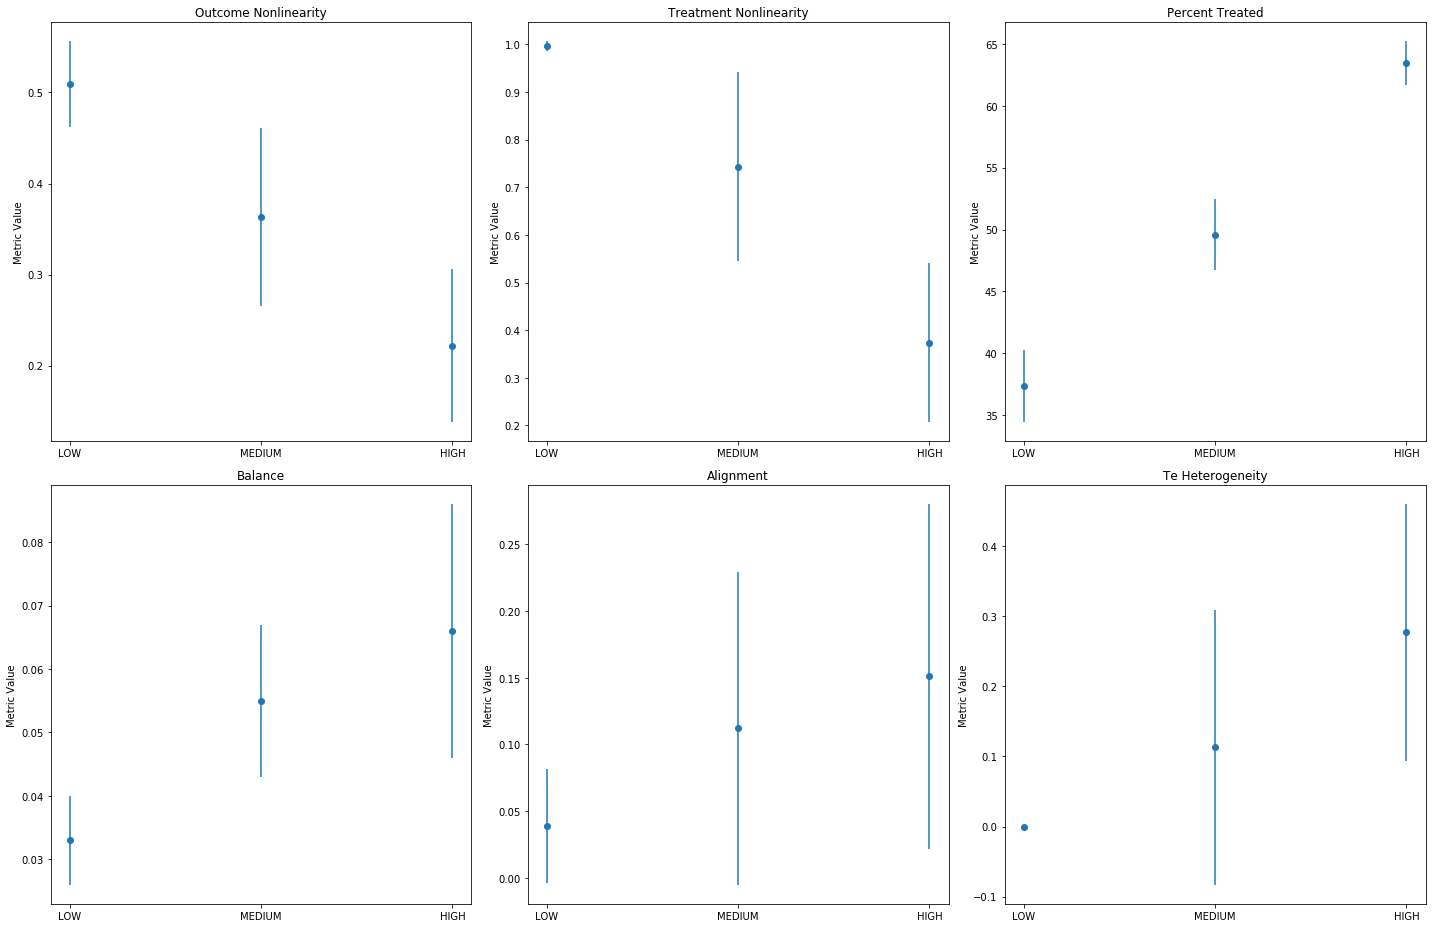
\includegraphics[width=1\linewidth]{figures/ch7-sampling-validation-1.png}
    \caption{DGP sampling parameterization validation results - data metric values (Y axis) for DGPs that are sampled at different `levels' (X axis) of each axis of the distributional problem space.}
    \label{fig:sampling-validation-results-1}
\end{figure}

The plots indicate that the level-based specification provides reasonable control over the position of sampled DGPs along each distributional problem space axis. Across all axes, the mean of the metric value at each level increases/decreases in the direction expected given the change in level\footnote{Note that, for each axis, the meaning of low, medium, and high is taken from the natural semantic interpretation of a low, medium and high level of that axis. So, for example, low imbalance means a more imbalanced covariate distribution in the treatment and control group, while a low outcome nonlinearity means a more linear outcome mechanism.}. Below, I describe the metric used to measure each value; see Chapter \ref{chap:macdesign} for a thorough theoretical introduction to the construction of these metrics. Working from top-left to bottom-right:

\begin{itemize}
    \item \textbf{Outcome Nonlinearity} measured by the $R^2$ value of a linear regression of the observed outcome on the observed covariates. The value of this metric decreases as the level of the axis is changed from low to high, as would be expected under decreasing linearity of the outcome mechanism.
    
    \item \textbf{Treatment Assignment Nonlinearity} measured by the $R^2$ value of a linear regression of the oracle treatment probability logit on the observed covariates. The value of this metric decreases as the level of the axis is changed from low to high, as would be expected under decreasing linearity of the treatment assignment mechanism.
    
    \item \textbf{Percent Treated} measured by the percent of units in the treated group. The value of this metric increases, as expected, as the percent treated axis level is changed from low to high.
    
    \item \textbf{Imbalance} measured by the Wasserstein Distance\footnote{The Wasserstein Distance is an \textit{integral probability metric} that measures the absolute value of the difference between the CDF of each distribution, integrated across the domain. This can be approximated by formulating a minimum flow optimization problem using the observed covariate values in each group. See the implemented metric code for detailed documentation.} between the covariate distributions in each treatment group. A higher metric value (larger Wasserstein Distance) indicates a larger distance between the distributions in each group, meaning greater imbalance. The values of this metrics increase, as expected, as the imbalance axis level is changed from low balance to high balance. 
    
    \item \textbf{Alignment} measured by linear regression of the observed outcome on the oracle treatment probability logit. A higher value of the metric means there is greater overlap in covariates between the treatment and outcome mechanisms. The values of the metric increase, as expected, as the alignment axis level is changed from low to high.
    
    \item \textbf{Treatment Effect Heterogeneity} measured by the ratio of the standard deviation of the treatment effect to the standard deviation of the observed outcome. The values of the metric increase as the axis level is changed from low to high, indicating an increasing portion of the individual outcome variance stems from changes in the treatment effect between individuals.
\end{itemize}

Note that, despite the promising trend in the mean of each metric, there is an evident weakness visible in the plots: The variance of the sampling process appears to be substantial relative to the scale of the differences in the (mean) metric values at each level. Some of this variance may be equivalent to \textit{measurement} noise\footnote{This noise could stem from the imprecise nature of the metric calculations and the stochasticity of the data sampled from each DGP.} rather than variance in the DGP sampling process itself. This can be tested by increasing the number of samples of data from each DGP to see if the standard deviation of the metric across DGPs decreases. Doubling the sample count from 100 to 200 does decrease the average standard deviation across all metrics and levels by about 30\%, which means that at least some of the variance can be attributed to measurement noise. However, even allowing for some measurement noise, it is likely that the source of at least some of the variance is the DGP sampling process itself. IE, at each parameterization, it is possible to sample DGPs which are quite dissimilar in their position along any given axis. This is confirmed by the analysis used to validate the benchmarking procedure below.

\section{Validating the Benchmarking Approach}

This section focuses on validating Maccabee's Hybrid Monte Carlo benchmarking approach. This is done by looking at a series of comparative cases that demonstrate key advantages. These cases are based on comparisons to the benchmarking approaches used in \textcite{Diamond2013GeneticStudies}. This paper was chosen because it benchmarks a new method for causal inference - Genetic Matching - using a series of three benchmarking approaches that align nicely with the landscape of approaches established in Chapter \ref{chap:litreview}. The benchmarking approaches used in the paper, categorized based on the ontology presented in Chapter \ref{chap:litreview}, are outlined below:

\begin{enumerate}
    \item \textbf{Pure, Synthetic Benchmarks}: First, \citeauthor{Diamond2013GeneticStudies} construct a series of synthetic DGPs based on the following scheme: Ten covariates are sampled from a joint distribution consisting of a mix of ten independent Bernoulli binary (with $p=0.5$) and standard normal variables. They specify a fixed outcome mechanism with a constant treatment effect. Finally, they hand-specify a set of seven treatment assignment (logit) functions (all generalized, additive functions) with escalating levels of nonlinearity (introduced through quadratic terms) and non-additivity (introduced through two-way interaction terms). This produces a total of seven synthetic DGPs labeled A-G in order of increasing treatment mechanism complexity.
    
    
    \item \textbf{Pure, Empirical Benchmark}: Second, \citeauthor{Diamond2013GeneticStudies} perform a pure empirical benchmark using the dataset from \textcite{Lalonde1986EvaluatingData}\footnote{See Chapter \ref{chap:macdesign} for a description of this dataset.}. The DGP in this case is unknown.
    
    
    \item \textbf{Hybrid Benchmark} Finally, the authors specify a hybrid benchmark that uses the covariates from the \textcite{Lalonde1986EvaluatingData} empirical benchmark and hand-specified treatment and outcome functions designed to produce data that `looks like' the empirical data from case two above. This conforms to the definition of a Hybrid Benchmark given in Chapter \ref{chap:litreview}.
\end{enumerate}

The results collected from these three different benchmarking approaches serve as a useful baseline against which results collected from Maccabee can be compared. With each of the three benchmarks providing insight into how different aspects of Maccabee's sampled-based Hybrid Monte Carlo approach improve the \textit{specific} and \textit{general} validity of the benchmarks and/or provide additional insight into estimator performance (compared to the Genmatch baseline)\footnote{See Chapter \ref{chap:litreview} for the definitions of specific and general validity.}. The sections below each focus on one of these comparisons. In each case, I customize the operation of the Maccabee package to provide as narrow a comparison as possible, maximizing the design aspects that are kept `constant' between the Genmatch and Maccabee approaches\footnote{It may be useful to the reader to conceptualize each of the original Genmatch benchmarks as providing a \textit{counterfactual} against which some (hopefully) improved aspect of Maccabee's approach can be compared to infer the effect of the change in approach. For example, case one tests the effect of sampling DGPs by comparing sampled vs. concrete DGPs that are entirely synthetic.}. The narrowness of the comparison is progressively relaxed across the three cases, with the results from the prior, narrower cases supporting the new, broader comparison in each case.

\vspace{\baselineskip}

\textbf{Note:} My original intention was to replicate all three benchmarking approaches from \textcite{Diamond2013GeneticStudies}, as described above, and then benchmark a few of the estimators that are compared in that paper. The analysis and results presented below are dramatically scoped down. I replicate only the first benchmarking approach, targeted at validating sampled-DGP-based benchmarking. Further, the only estimator that is benchmarked is the Logistic Propensity Matching Estimator - the baseline estimator in \textcite{Diamond2013GeneticStudies}. This is enough to validate the core contribution of the approach proposed in this paper. I present the (experimental) design that would be used to implement the validation based on the other two benchmarking approaches. This is done in order to guide future work and highlight the aspects of Maccabee's design that are not validated by the results presented below. Future work will collect results for the last two cases and extend all three cases to include results from the range of estimators that appear in \textcite{Diamond2013GeneticStudies}.

\subsection{Sampled vs Static Synthetic DGPs}
\label{sec:comparison-1}

This section focuses on validating the idea of sampling treatment assignment and outcome mechanisms in the (simple) context in which these mechanisms are defined over synthetic covariate data. This is done by comparing a sample-based, synthetic DGP benchmark, executed using Maccabee, to \citeauthor{Diamond2013GeneticStudies}'s static, synthetic benchmarking approach - approach one above. Both of these benchmarking approaches are `pure', in the ontology from Chapter \ref{chap:litreview}, because the data and the treatment/outcome mechanisms are entirely synthetic. The only difference between the two approaches is in how the treatment/outcome mechanisms are constructed. This provides a narrow, and therefore useful, comparison. The goal of this comparison is to show that Maccabee produces benchmarks with greater \textit{specific validity} by capturing the distribution over estimator performance within a specific region of the distributional problem space. This is explained in greater detail below.

\subsubsection{Comparison Explanation}

In order to maximize the `constants' across the two approaches, the standard Maccabee benchmark is customized so that:

\begin{enumerate}
    \item The covariate observations are sampled from the same distribution as used in \textcite{Diamond2013GeneticStudies}.
    
    \item The sampled DGPs have the exact same outcome mechanism and (constant) treatment effect that are used in \textcite{Diamond2013GeneticStudies}.
    
    \item The sampled DGPs have a treatment assignment mechanism with the same functional form as the one used in Scenario G of the paper. IE, the low-level parameterization of the treatment assignment mechanism sampler is set to sample functions that look almost identical to the baseline treatment assignment mechanism from Genmatch. This means that the number of terms of each type - linear, quadratic, and two-way interaction - will be the same across sampled and hand-specified functions. The only source of variance is which covariates are selected for each term type and what coefficients are used. 
    
    \item The coefficients for the treatment assignment mechanism are sampled from a distribution designed to produce coefficients that are very similar to the ones in the hand-specified functions.
\end{enumerate}

Note that this is a much lower variance setting (in terms of variance over the sampled functions) than a standard Maccabee sampled benchmark. A standard sampled benchmark would sample a set of functions with varied functional forms, targeting a given level of nonlinearity. In this comparison, the samples are drawn from the set of functions with the exact same form as the hand-specified function. The implication of this fact is that variance in this class of functions is strictly less than the variance we would expect when sampling from the universe of possible functional forms.

\vspace{\baselineskip}

With the above established, the (compared) benchmarking procedures are as follows: In the original work, \citeauthor{Diamond2013GeneticStudies} sample 1000 datasets from the DGP in Scenario G and report the Root Mean Squared Error and the Absolute Bias (Percentage) of a number of estimators (including Genetic Matching)\footnote{See Chapter \ref{chap:macimplementation} for definitions of these performance metrics}. I repeat this data sampling thirty times to produce an interval that quantifies the variance of the performance metrics for this single DGP. In order to construct the comparison benchmark, I sample 16 DGPs and, from each, sample 1000 datasets, 30 times\footnote{In the language of Maccabee, this is 16 sampled DGPs with 30 sampling runs of 1000 datasets each.}. This produces a set of 16 performance metric intervals for comparison with the single hand-specified DGP interval. On top of the performance metrics, I also collect the data metrics for all data sets to allow for a comparison and analysis of the concrete/sampling DGP distributional setting.

\subsubsection{Comparison Implementation}

All of the above is done using Maccabee. The hand-specified DGP from \textcite{Diamond2013GeneticStudies} is sampled using a custom, concrete DGP, and the sampled DGPs are constructed using the default Maccabee sampler with custom parameters, a custom data source and a customized DGP class (to keep the outcome mechanism fixed)\footnote{See Chapter \ref{chap:macimplementation} for explanations of these implementation concepts.}. The case study code is available in a Notebook \href{https://github.com/JoshBroomberg/Maccabee/blob/master/Notebooks/Genmatch\%20Benchmarking\%20Validation.ipynb}{here}. 

\vspace{\baselineskip}

The two highly specific benchmarking schemes - one for the customized sampling procedure and one to replicate the benchmark in \textcite{Diamond2013GeneticStudies} - are implemented with no changes to the underlying package code. IE, any external user of the package could replicate this validation using only the user-facing tools provided by the package. This is a testament to the flexibility provided by Maccabee's design and implementation.

\subsubsection{Comparison Results}

Table \ref{tbl:pure-synth-data-metrics-1} displays the average data metric values for the datasets produced by the Genmatch and Maccabee (sampled) DGPs. The metric values are close to identical for all metrics. This does not mean that all the sampled DGPs have the same metric value (this variance will be discussed shortly), but it does mean that the concrete treatment assignment mechanism selected in the Genmatch paper appears to be a `typical' function in the set of functions of the same form. Typical, in this setting, means that the metric values for the selected function match the mean of the metric values for the DGPs constructed by sampling from the set of all functions of the same form.


\begin{table}[ht!]
\centering
    \begin{tabular}{|l|l|m{1.5cm}|m{1.5cm}|}
    \hline
    \rowcolor[HTML]{EFEFEF} 
    Axis & Metric & Genmatch Value & Maccabee Value \\ \hline
    Outcome Nonlinearity & Lin r2(X\_obs, Y) & 0.909 & 0.905 \\ \hline
    Outcome Nonlinearity & Lin r2(X\_true, Y) & 0.91 & 0.907 \\ \hline
    Outcome Nonlinearity & Lin r2(X\_obs, Y0) & 1.0 & 1.0 \\ \hline
    Outcome Nonlinearity & Lin r2(X\_true, Y0) & 1.0 & 1.0 \\ \hline
    Treatment Nonlinearity & Lin r2(X\_obs, Treat Logit) & 0.938 & 0.796 \\ \hline
    Treatment Nonlinearity & Lin r2(X\_true, Treat Logit) & 1.0 & 1.0 \\ \hline
    Treatment Nonlinearity & Log r2(X\_obs, T) & 0.679 & 0.669 \\ \hline
    Percent Treated & Percent(T==1) & 54.927 & 50.309 \\ \hline
    Alignment & Lin r2(Y, Treat Logit) & 0.059 & 0.1 \\ \hline
    Alignment & Lin r2(Y0, Treat Logit) & 0.014 & 0.096 \\ \hline
    Alignment & Log r2(Y0, T) & 0.552 & 0.612 \\ \hline
    Alignment & Log r2(Y, T) & 0.665 & 0.669 \\ \hline
    Treat Effect Heterogeneity & std(TE)/std(Y) & 0.0 & 0.0 \\ \hline
    \end{tabular}
    \caption{Data metrics values for DGPs produced for the comparison between the Genmatch and Maccabee benchmarks based on pure, synthetic DGPs. Maccabee produces sampled DGPs with mean metric values that are close to the metric values for the original Genmatch DGP. This indicates that the concrete Genmatch DGP is a `typical' relative to the the restricted set of functions of similar form. For guidance on interpreting the metrics (and metric naming scheme) in this table, see Section \ref{sec:measuring-distributional-setting} of Chapter \ref{chap:macdesign}.}
    \label{tbl:pure-synth-data-metrics-1}
\end{table}
\FloatBarrier

Based on the similar average data metrics, one would expect that the mean performance of the causal estimator on the data from the Genmatch vs. sampled Maccabee DGPs would be similar (if the data metrics are predictive of performance). Indeed, this appears to be the case. Comparing the values of the two performance metrics used by \citeauthor{Diamond2013GeneticStudies}:

\begin{itemize}
    \item The Mean Absolute Bias Percentage (MABP) is 7.592\% (std 0.11\%) in the Genmatch benchmark and 7.054\% (std 1.24\%) in the Maccabee benchmark.
    
    \item The Root Mean Squared Error is 0.038 (std 0.001) in the Genmatch benchmark and 0.035 (std 0.006) in the Maccabee benchmark.
\end{itemize}

At this point, the only evident difference between the two benchmarking approaches is the standard deviation of the Mean Absolute Bias Percentage performance metric. Upon closer examination, this turns out to be crucially important. Figure \ref{fig:benchmark-validation-pure-synth-1} shows the distribution over performance metric values in the sampled DGPs compared to the performance metric value/s for the concrete, Genmatch DGP. It is clear, from both panels in the figure, that the MABP value for the Genmatch DGP is (fairly typical) `sample' from a \textit{distribution} over the performance metric. The variance in this distribution is driven primarily by estimator performance differences across between different, sampled DGPs rather than the variance of the estimator \textit{within} each DGP (when applied to datasets sampled from the DGP). This is initial evidence for the importance of evaluating estimators based on sampled DGPs that capture information on the complete distribution of performance metric values rather than evaluating based on a single sample from this distribution.

\vspace{\baselineskip}

Concretizing this idea with respect to the case study at hand, observe that all of the sampled functions have the same structure/form as the concrete, hand-specified function in the paper. It is thus conceivable/likely that any of the sampled functions could have been selected, producing a single sample from the performance distribution presented in Figure \ref{fig:benchmark-validation-pure-synth-1}. In the example above, the empirical (bootstrapped) interval containing 95\% of the probability mass is bounded between 5.5\% to 9.7\% MABP. This (roughly) implies that 95\% of the single performance values produced by hand-specified DGPs would fall into this interval. In absolute terms, the size of this interval is appreciable. But the absolute size is not as important as the size relative to a) differences in the (mean) performance of different estimators or b) relative to the corresponding intervals for other estimators (distributional overlap). If the performance metric distribution for one estimator overlaps with the performance metric distribution for a second estimator, then the rate of false ordinal ranking from point comparisons of estimator performance metrics (based on single samples) will be proportional to the degree of overlap in the distribution. Without access to/quantification of this overlap, or at least to the variance of the distribution, the error rate of the point comparisons is entirely unknowable. In this state of knowledge, even large absolute differences in performance - which are normally treated as strong evidence of estimator superiority - may actually represent weak evidence of superior relative performance (if the variance is large).

\vspace{\baselineskip}

The results presented in Figure \ref{fig:benchmark-validation-pure-synth-1} above show that this variance exists even within a very narrow class of DGP functional forms, all targeting one region of the distributional problem space. On a wider/more complete set of functional forms, targeting more of/all of the problem space, there is likely to be appreciably more variance in performance. Given this, accurately characterizing/comparing estimator performance requires understanding the \textit{distribution} over estimator performance rather than relying on single-sample point estimates. I return to this point below after a brief digression to bring the measured values of the data metrics into the discussion.

\begin{figure}[ht!]
    \centering
    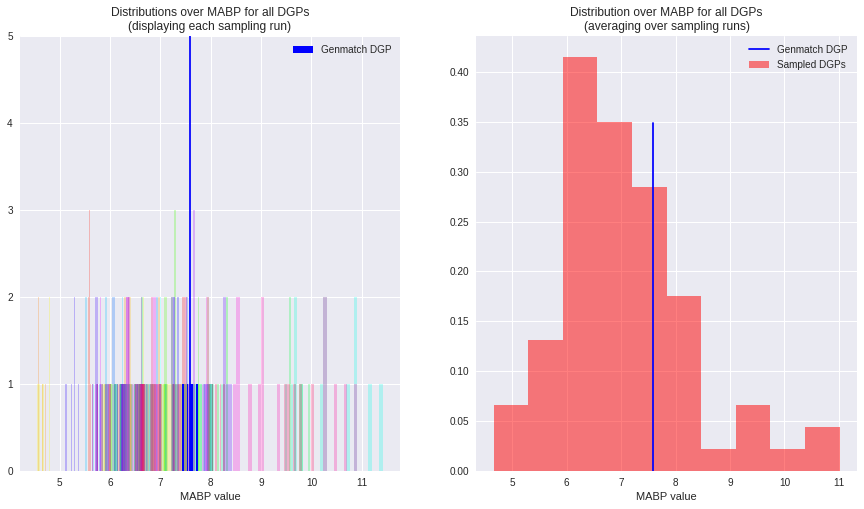
\includegraphics[width=1\linewidth]{figures/ch7-benchmark-pure-synth-1.png}
    \caption{Performance metrics values for the Logistic Propensity Matching estimator applied to DGPs produced by for comparison between the Genmatch and Maccabee benchmarks based on pure, synthetic DGPs. The performance of the estimator on the concrete DGP from the Genmatch paper is a typical sample from a distribution over possible performance metrics generated by sampled DGPs with almost identical functional form. Left panel: the distribution over the Mean Absolute Bias Percentage for each DGP, based on the sampling runs for the DGP. Each sampled DGP is in a different color. The concrete, Genmatch DGP in blue. This is a distribution over distributions. The variance of performance between DGPs is much larger than the variance within DGPs. Right panel: the distribution over the mean value of the performance metric across all sampling runs for each DGP.}
    \label{fig:benchmark-validation-pure-synth-1}
\end{figure}
\FloatBarrier

The natural question to ask at this point, given the discussion in previous chapters, is how the performance metrics discussed above are correlated to the data metrics which measure the location of DGPs/generated data in the distributional problem space. Figure \ref{fig:benchmark-validation-pure-synth-2} shows the MABP performance metric plotted against a metric that measures treatment nonlinearity. This plot is interesting. Firstly, while there is a clear (and significant, with p=0.0001) correlation, this correlation is reversed from what we would expect. One would expect that as the linearity increases (with higher values of the metric corresponding to increased linearity), the performance of the Logistic Propensity Matching estimator - which estimates propensity scores using a linear model - would improve. However, the reverse appears to be true. The reason for this is discussed shortly.
\vspace{\baselineskip}

Regardless of the trend direction, there are two important observations.

\begin{enumerate}
    \item Even within a narrow set of functions, there is variance in the position of DGPs in the distributional problem space as measured by data metrics. This variance is significant in that it is meaningfully correlated with changes in the performance of estimators. This means that choosing a single DGP from the set of possible DGPs is risky as it could appear anywhere in the distribution over the possible distributional setting and hence anywhere in the distribution over estimator performance.
    
    \item Even though the data metric is predictive of performance, there is still significant variance in the performance metric at each data metric. This implies that even DGPs with similar measurable distributional settings on one axis may differ in other performance-relevant axes.
\end{enumerate}

Both of these points imply that sampling benchmarking DGPs, to produce a sample the distribution of performance metrics for a given estimator, is crucial. DGPs with a fixed functional form can cover a meaningful range of distributional settings and, within each setting, there is still variance in performance. Given this variance, metrics calculated over sampled performance metric distributions - the mean or median, for example - provide a much clearer picture of the performance of an estimator in a region of the problem space than the picture provided by a single sample. Using a single DGP (to produce a single sample) risks using an arbitrary location in the distribution to characterize performance without any consideration for the shape of the underlying distribution from which this value is drawn.

\vspace{\baselineskip}

The first point - that there is a correlation between performance and the measured data metrics - also motivates an approach that targets specific locations in the distributional problem space. If the location in the distributional problem space (as measured by the data metrics) is indeed predictive of estimator performance, then accurate evaluation of performance requires benchmarking under all, or known, distributional settings in the space. Failure to consider the location of the benchmarking data in the distributional problem space is, analogously to the failure above, like judging the performance of an estimator based on a single `sample'. There is little apriori reason to believe that an estimator that is superior in one location in the distributional problem space will be superior in all locations of interest.

\begin{figure}[ht!]
    \centering
    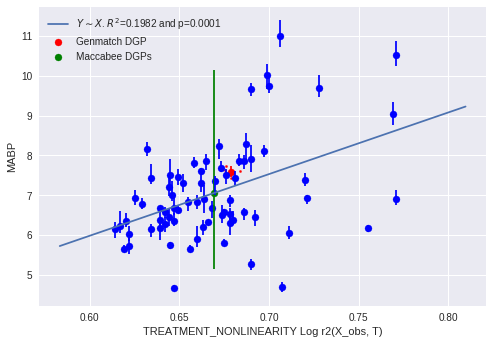
\includegraphics[width=0.9\linewidth]{figures/ch7-benchmark-pure-synth-2.png}
    \caption{Pure, Synthetic benchmark performance metric plotted against the data metric values for treatment nonlinearity. Maccabee sampled DGPs are in blue with the blue dot at the mean performance and data metric value for each sampled DGP and error bars corresponding to the standard deviation of the performance metric across the sampling runs for the DGP. The concrete, Genmatch DGPs are in red with a large red dot at the mean performance/data metric value and an individual, smaller dot for the performance/data metric value of each sampling run. It is clear that the treatment nonlinearity metric is predictive of performance but only explains a small portion of the variance in the performance. It is also clear that the concrete Genmatch DGP displays performance which is typical of its treatment nonlinearity.}
    \label{fig:benchmark-validation-pure-synth-2}
\end{figure}
\FloatBarrier

Returning to the reversed-from-expectation direction of the trend in Figure \ref{fig:benchmark-validation-pure-synth-2}. A hypothesis that would explain this observation is that the more linear the treatment function, the more alignment there is between the treatment and outcome functions (because the outcome function is linear). As established in Chapter \ref{chap:litreview}, this would then mean there is a larger degree of confounding to reverse. This hypothesis appears to be borne out by the data presented in Figure \ref{fig:benchmark-validation-pure-synth-3}. This figure, which is directly analogous to Figure \ref{fig:benchmark-validation-pure-synth-2}, displays the MABP performance plotted against a metric that measures alignment. It shows that as alignment increases, the MABP increases. Further, there is a strong correlation between the metric used to measure treatment nonlinearity (from Figure \ref{fig:benchmark-validation-pure-synth-2}) and the metric used to measure alignment (from Figure \ref{fig:benchmark-validation-pure-synth-3}), with an $R^2$ of $0.4$ and a p-value $< 10^{-5}$ \footnote{A plot of the relation between these metrics is included in the notebook linked above}. Ironically, given the subject matter of this paper, it is hard to resolve the causality that relates these interlinked trends. It is plausible that the alignment created by increased linearity in the treatment mechanism increases the error in causal inference enough to mask/mitigate the increase in accuracy produced by the (more) correct specification of the treatment assignment model\footnote{Recall that the estimator being used matches on a linear propensity model.}.

\vspace{\baselineskip}

This raises another, more subtle concern with hand-specified benchmarks. Hand-specification may target DGPs based on various levels/positions along one or more axes of the distributional problem space but, without additional effort, may not pay attention to the position of the specified DGP along other, performance-relevant axes. For example, the analysis above implies that \textcite{Diamond2013GeneticStudies} may underestimate the accuracy of estimators in their high nonlinearity setting by inadvertently introducing increased alignment with the fixed, linear outcome mechanism. Maccabee's principled approach to DGP generation forces researchers to pay attention to the location of sampled DGPs on all axes. This, combined with the metrics that measure distributional setting (and enable analyses of the kind above), should help to mitigate this kind of specification issue.

\begin{figure}[ht!]
    \centering
    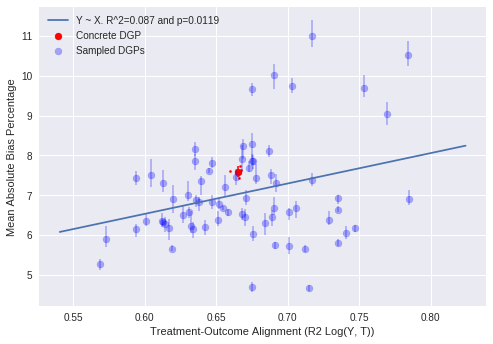
\includegraphics[width=0.9\linewidth]{figures/ch7-benchmark-pure-synth-3.png}
    \caption{Pure, Synthetic benchmark performance metric plotted against the data metric values for treatment-outcome alignment. As in Figure \ref{fig:benchmark-validation-pure-synth-2}, Maccabee sampled DGPs are in blue with the blue dot at the mean performance and data metric value for each sampled DGP and error bars corresponding to the standard deviation of the performance metric across the sampling runs for the DGP. The concrete, Genmatch DGPs are in red with a large red dot at the mean performance/data metric value and an individual, smaller dot for the performance/data metric value of each sampling run. The graph displays a similar trend to the one in Figure 2 - as alignment increases, the MABP increases. This is the expected direction of this trend, given the theory outlined in Chapter \ref{chap:problemspace}. It is possible that the unexpected trend direction from Figure \ref{fig:benchmark-validation-pure-synth-2} results from the fact that, in this case, increased treatment linearity increases alignment, which could increase the difficulty of causal modeling enough to mask the gain in accuracy from the treatment linearity.}
    \label{fig:benchmark-validation-pure-synth-3}
\end{figure}
\FloatBarrier

\subsection{Sampled Hybrid DGP vs. Static Hybrid DGP}

This section focuses on validating the idea of sampling treatment assignment and outcome mechanisms when these mechanisms are defined over (complex) empirical covariate data. This is done by comparing a sample-based, hybrid DGP benchmark, defined over the \textcite{Lalonde1986EvaluatingData} data and executed using Maccabee, to \citeauthor{Diamond2013GeneticStudies}'s static, hybrid benchmarking approach - approach two above. Both of these benchmarking approaches are `hybrid', in the ontology from Chapter \ref{chap:litreview}, because the data is empirical while the treatment/outcome mechanisms are synthetic. The goal of this comparison is to validate the sampling approach when:

\begin{enumerate}
    \item The covariate data, over which the sampled mechanisms are defined, is non-ellipsoidal, skewed, or otherwise degenerate. IE, the kinds of covariate data seen in empirical settings.
    
    \item The DGP sampling parameterization is used to target a region of the distributional problem space rather than sampling instantiations of a specific functional form as was done in case one above.
\end{enumerate}

The comparison here can, thus, be thought of as an extension of the comparison presented in Section \ref{sec:comparison-1} above. The goal is the same: to show that Maccabee produces benchmarks with greater \textit{specific validity} by capturing the distribution over estimator performance within a specific region of the distributional problem space. But now in a more complex and, therefore, realistic benchmarking setting. Logically, a positive result would be achieved in this comparison if it were to produce similar results to the ones presented above. This would demonstrate that Maccabee can target the same region of the problem space targeted by a (complex) manually-specified design defined over empirical covariates while recovering a distribution over estimator performance rather than a point estimate. It is worth emphasizing that the point of this comparison is not to generate \textit{different} results than those presented in \textcite{Diamond2013GeneticStudies} but rather to show that the benchmark results in that paper are a \textit{single sample} from a distribution over estimator performance in the selected region of the problem space.

\subsubsection{Comparison Explanation and Implementation}

As noted above, this comparison is not actually implemented. This subsection provides a brief overview of how it should be implemented in future work.

\vspace{\baselineskip}

The difference between the two approaches compared in this section is, again, in how the treatment/outcome mechanisms are constructed. \textcite{Diamond2013GeneticStudies} construct the treatment assignment and outcome mechanisms to produce a setting that is designed to be `difficult' for any causal estimator. This is done by manually crafting mechanisms, defined over the empirical data, that exhibit properties known to be challenging for methods of observational causal inference. Quoting the salient components of the design write up:

\begin{quote}
    (Outcome mechanism) ...the mapping from baseline covariates to Y is obviously non-linear and only two of the baseline variables are directly related to Y.
\end{quote}

\begin{quote}
    (Treatment assignment mechanism) ...this propensity score is a mix of the estimated propensity score in the Dehejia and Wahba sample plus extra variables in Equation 4, because we want to ensure that the propensity model estimated in the Monte Carlo samples is badly misspecified.
\end{quote}

In contrast to this, Maccabee's treatment and outcome mechanisms are sampled based on sampling parameters. These parameters can be specified to create similarly difficult distributional setting \textit{without directly specifying the two mechanisms}. This is possible because the Maccabee specification of (sampled) DGPs is given in terms of a region in the distributional problem space rather than as a specific DGP (that exists in some location in the space). Observe that this is not fundamentally different from the approach taken by \citeauthor{Diamond2013GeneticStudies}. The authors do, in fact, consider the distributional problem space, implicitly and explicitly, to inspire the design of the specific DGP used in their benchmark. For example, in the first quote above, the authors reference the nonlinearity of and the number of covariates included in the outcome mechanism. These concepts are directly related to axes of the distributional problem space, as established in Chapter \ref{chap:problemspace}. Maccabee simply allows the benchmark to be expressed in terms of the desired location in problem space directly with requiring the choice of a single instantiation.

\vspace{\baselineskip}

Maccabee has all of the DGP sampling parameters required to sample DGPs from the region of problem space targeted by \textcite{Diamond2013GeneticStudies}. The following rough sampling parameterization should be used:

\begin{itemize}
    \item The \texttt{potential confounder selection} probability should be set so that the number of useful/predictive covariates (those that enter the sampled treatment and outcome mechanisms) is equal, in expectation, to the number used in \textcite{Diamond2013GeneticStudies}.
    
    \item The \texttt{treatment/outcome nonlinearity} parameters should be set to generate treatment and outcome mechanisms with nonlinearity that matches the nonlinearity of these mechanisms in \textcite{Diamond2013GeneticStudies}. Unlike in the case above, this should be done without targeting the exact functional forms used in \textcite{Diamond2013GeneticStudies}. Rather, it should be achieved using Maccabee's built-in parameter specification and optimization tools (as described in the documentation, \href{\RTDurl/usage/custom-sampled-dgp.html}{here}). These tools can be used to target the same measurable level of nonlinearity as in the mechanisms from the original paper. This is all that should be required\footnote{\citeauthor{Diamond2013GeneticStudies} include an estimated propensity score, produced by the propensity model that will be used in the benchmarked estimators, in the treatment assignment mechanism. This is designed to ensure that the propensity model is ``badly misspecified''. This is likely unnecessary in Maccabee (although it could be achieved by customizing the sampled DGP). The size of the universe of possible propensity functions that can be sampled means that the fixed propensity score model proposed in \textcite{Diamond2013GeneticStudies} is highly likely to be misspecified.}.
    
    \item The \texttt{treatment probability} parameter should be set to mimic the bimodal treatment probability distribution outlined in \textcite{Diamond2013GeneticStudies}.
    
    \item The \texttt{treatment effect heterogeneity} parameter should be set to ensure a constant treatment effect.
\end{itemize}

A positive result would look much like the results presented above. The Genmatch benchmark result should, ideally, present as a single sample from a distribution of estimator performance. A priori, I would expect this performance distribution to be wider in this case given the relaxed constraints on the DGP sampling process\footnote{IE, sampling of both treatment and outcome mechanisms and matching the Genmatch design based on measured data metric values rather than specific functional form.}.

\subsection{Sampled Hybrid DGP vs. Empirical DGP}

This section focuses on validating the hybrid benchmarking approach by comparing it to a standard empirical benchmark of the kind that is common in the literature. This is done by comparing a sample-based, hybrid DGP benchmark, defined over the \textcite{Lalonde1986EvaluatingData} data and executed using Maccabee, to \citeauthor{Diamond2013GeneticStudies}'s empirical benchmarking approach - approach three above. Of the three comparisons, this one involves the least obvious comparison. Its goal is to establish Maccabee's ability to improve \textit{general validity} by evaluating the performance of causal estimators on observational data from across the distributional problem space while preserving the realism of the data generating processes used to generate the data. The comparison to a pure, empirical benchmark is chosen because, as established in Chapter \ref{chap:litreview}, this method is widely considered the gold-standard of \textit{realistic} benchmarking, but evaluates causal estimators at a single (unknown) location in the problem space. The goal of the comparison is, therefore, to show that Maccabee produces performance results similar to the empirical benchmark when the sampled DGPs are (measured to be) close to the empirical DGP in the problem space while also being able to sample the DGPs required to evaluate an estimator across the rest of the problem space (where the performance results are expected to be quite different).

\vspace{\baselineskip}

In this comparison, Maccabee should be configured and fine-tuned according to the best practices outlined in the \RTDlink{package documentation}\footnote{As pointed out in the documentation; it is important to fine-tune the sampling parameterization for the specific empirical covariates to ensure one is sampling from the intended region/s of the distributional problem space.}. It should then be used to sample DGPs from across the distributional problem space (perhaps sampling from all combinations of the three, predefined levels of each of the problem space axes).

\vspace{\baselineskip}

A positive result would be one in which estimator performance varies across the sampled DGPs. With the DGPs most similar to the empirical `DGP' (data), in terms of the values of the data metrics that quantify position in the problem space, exhibiting similar estimator performance to the estimator performance on the empirical `DGP'. This would demonstrate that the empirical DGP benchmark used in the paper effectively evaluates causal estimators in a single region of the distributional problem space and that this (unknown) location has an important effect on the observed performance. Relative to this, Maccabee provides a way to evaluate estimator performance across the distributional problem space without greatly sacrificing \textit{specific validity} (as established by the two cases above).

\section{Conclusion}

The results presented in this chapter provide initial validation of the Maccabee's benchmarking approach and implementation. The first section demonstrated that Maccabee's sampling parameterization could be used to control the (measured) location of DGPs in the distributional problem space. The second section used a series of comparative cases to validate different aspects of Maccabee's benchmarking approach. This was done by comparing the results from Maccabee benchmarks to the benchmarking results from \textcite{Diamond2013GeneticStudies}. The first case in this section established that sampling only one component of the benchmarking DGP, while preserving a fixed functional form, produced appreciable variance in estimator performance measured using the sampled DGPs. This observation motivates for the importance of using sampled DGPs to produce (large) samples from the estimator-specific distribution over performance metric values. The results in this first case also provided initial evidence for the relation between the location in the distributional problem space and observed estimator performance, motivating DGP sampling that controls for this location. The second and third cases were proposed but not executed. The second case is designed to extend the results from the first case to more realistic covariate data. The third case is designed to provide further evidence for the importance of knowing and/or controlling the location of (sampled) benchmarking DGPs in the distributional problem space.

\end{document}